\chapter{Bytecode Manipulation}


\section{Java Classes}
\subsection{Structure of Class}
The overall structure of a compiled java class is very simple, and it retains structural information and symbols from source code. As described in [21], the compiled class consists of:
\begin{itemize}
\item The section that describes the name, the modifiers, the interfaces, the super class and the annotations of the class.
\item A section for each field, which describes the modifiers, name, type and annotations of the field. 
\item One section for each method and constructor that are declared within the class. This section describes the modifiers, the return type and  parameter types, annotations and name for the constructor or method. The compiled code of the method is also included as a sequence of java bytecode instructions.
\end{itemize}

A compiled class consists of a constant pool section, which is an array of the numeric, type and string constants that appear within a class [21]. These constants are defined only once, and are referenced in all the other sections using their index. The figure below from [21] shows the overall structure of a compiled class:

\begin{figure}[htb]
\centering
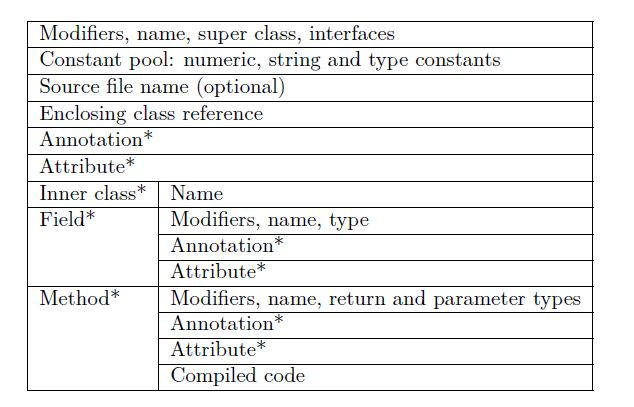
\includegraphics[width=0.6\textwidth]{images/class_structure.jpg}
\caption{Overall structure of a compiled class(* means zero or more)} 
\label{fig: Overall structure of a compiled class(* means zero or more)}
\end{figure}  
\break

Java types are represented i a different way in compiled class than the source class. Consider, superclass of a class, or exceptions thrown by a method cannot be primitive or array types. They can only be class or interface types, and hence are represented with internal names. For example, java/lang/String is the internal name for String. 

Type descriptors are used for representing field types. the following figure taken from [21] represents type descriptors for some Java types:

\begin{figure}[htb]
\centering
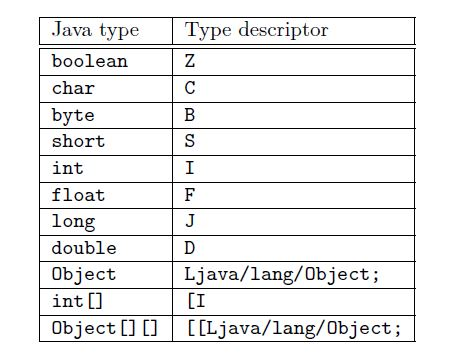
\includegraphics[width=0.6\textwidth]{images/type_desc.jpg}
\caption{Type descriptors of some Java types} 
\label{fig: Type descriptors of some Java types}
\end{figure} 
\break

The descriptors of primitive types are single characters, class type are internal name of class, followed by a semicolon and preceded by L. The descriptor of an array is a square bracket, followed by array element type. 

A method descriptor consists of list of type descriptors which include parameter and return type of a method. Some sample method descriptors as represented in [21] are :

\begin{figure}[htb]
\centering
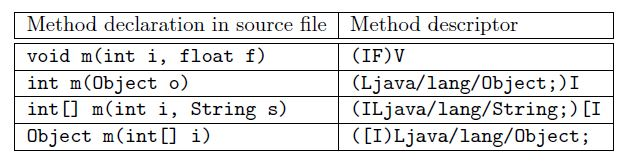
\includegraphics[width=0.6\textwidth]{images/method_des.jpg}
\caption{Sample method descriptors} 
\label{fig: Sample method descriptors}
\end{figure}
\break

\subsection{Structure of Method}
A method code is stored as a sequence of bytecode instructions inside a compiled class. Bytecode is the intermediate representation of Java programs just like assembler being the intermediate representation for C or C++programs [9]. The figure below shows the overview of a java program execution and where bytecode resides in the entire process [29]: 

\begin{figure}[htb]
\centering
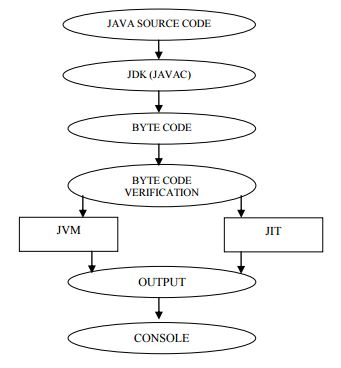
\includegraphics[width=0.8\textwidth]{images/jvm.jpg}
\caption{Java program execution} 
\label{fig:Java program execution}
\end{figure}
\break

To understand the bytecode thoroughly, we must understand the internal execution process of Java Virtual Machine (JVM). A JVM is a stack-based machine [9]. Each thread has a JVM stack which stores frames. A frame is created each time a method is invoked, and consists of an operand stack, an array of local variables, and a reference to the run-time constant pool of the class of the current method. Conceptually, it might look like this [9]:

\begin{figure}[htb]
\centering
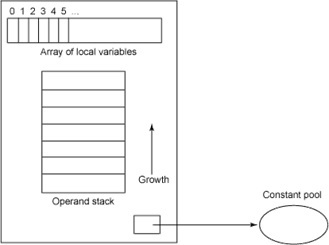
\includegraphics[width=0.6\textwidth]{images/frame.jpg}
\caption{JVM bytecode execution} 
\label{fig:JVM bytecode execution}
\end{figure}
\break

The local variable table or the array of local variables, consists of the parameters of the method and is used for holding the values of the local variables. Beginning at index 0, the parameters are stored first. Location 0 holds the reference, if the frame is for instance method or constructor. It is followed by location 1 which contains the first formal parameter, location 2 the second, and so on. For a static method, the first formal method parameter is stored in location 0, the second in location 1, and so on [9].

The size of the local variable table is determined at compile time, depending on the number and size of local variables and formal method parameters. The operand stack is a LIFO stack used to push and pop values, whose size is also determined at compile time. Certain opcode instructions push values onto the operand stack; others take operands from the stack, manipulate them, and push the result. The operand stack is also used to receive return values from methods.

\subsection{Bytecode Instructions}
A bytecode instruction is made of two parts, opcode and arguments.
\begin{itemize}
\item The opcode is an unsigned byte value [21]. 
\item The arguments are static values that are used for defining the instruction behavior [21].
\end{itemize}

The bytecode instructions can be divided in mainly two categories: one that are used for exchange of values between local variables and the operand stack; the others only work on the operand stack. They are used for computation of results, popping and pushing values on the stack. 

In this paragraph, we discuss the first kind of bytecode instructions that are used to load and store from local variables and operand stack. The ILOAD, ALOAD, FLOAD, LLOAD and DLOAD instructions are used for reading a local variable and pushing its value on the operand stack [21]. The index i of the local variable is taken as the argument. LLOAD, FLOAD and DLOAD are used for loading long, float and double respectively. ILOAD is used for loading of boolean, char, byte, int, or short local variable. The non-primitive values, which are objects and array references are loaded using ALOAD. In a similar way, ISTORE, FSTORE, LSTORE, ASTORE and DSTORE are used to pop values from operand stack and store them back to the local variable at index i.

The next set of instructions are those that work on operand stack only. The can be grouped as follows [21]:

\begin{itemize}
\item Stack - All possible instructions that can be used for manipulation of values on stack come under this category : POP, SWAP, DUP, PUSH, etc.
\item Constants - A constant value is pushed on the operand stack by these instructions. For example, ICONST{\_}0 pushes int value 0, FCONST{\_}0 pushes 0f, ACONST{\_}NULL pushes null, LDC cst pushes the arbitrary float, long, double, int, class or String constant cst, etc.
\item Arithmetic and Logic - These instructions do not have any argument and are used for performing arithmetic and logical operations on values, by popping them from the operand stack. After performing the operations, the result is pushed back on the operand stack. The operations include xADD, xSUB, xDIV, xREM and xMUL, where x is either I, L, D or F [21]. 
\item Casts -  These instructions are used for typecasting operations like I2F, L2D, F2D, etc. which are converting from one numeric type to another. 
\item Objects - These instructions are used for creation and locking of new objects. For example, NEW \textit{type} pushes a new object on the stack, where type is an internal name.
\item Fields - These instructions are used for reading or writing the values of the field. GETFIELD \textit{owner name desc} pops an object reference, and pushes the value of its name field. In a similar way, PUTFIELD \textit{owner name desc} pops a value and an object reference, and stores this value in its name field.
\item Methods - These instructions are used for invoking a constructor or a method. These instructions first pop values same as the the number of method arguments and one extra for the target object, to push the result. INVOKEVIRTUAL, INVOKESTATIC, INVOKESPECIAL, INVOKEINTERFACE, etc. are used for invoking different kinds of methods and constructors.
\item Arrays - Reading and writing of values in arrays is performed by these instructions. Some instructions are xALOAD, xASTORE, where x can be I, F, L, D, A, B, C, S.
\item Jumps - Jumps are used to go to an arbitrary instruction on occurrence of certain condition. Examples of these instructions include IFNE, IFGE, TABLESWITCH, etc.
\item Return - RETURN and xRETURN are used to return the result and terminate the method. RETURN is used for void return type and xRETURN for others.  
\end{itemize}

Let us consider an example given in [21], to get clear understanding:
\begin{verbatim}
public void checkAndSetF(int f) {
    if (f >= 0) {
       this.f = f;
    } else {
       throw new IllegalArgumentException();
    }
}
\end{verbatim}

The bytecode for this method is :
\begin{verbatim}
   ILOAD 1
   IFLT label
   ALOAD 0
   ILOAD 1
   PUTFIELD pkg/Bean f I
   GOTO end
label:
   NEW java/lang/IllegalArgumentException
   DUP
   INVOKESPECIAL java/lang/IllegalArgumentException <init> ()V
   ATHROW
end:
   RETURN
\end{verbatim}

The first instruction pushes the local variable 1, which is initialized to f, on the operand stack. The next instruction, IFLT pops this value from the operand stack, and compares it to 0. If the value is Less Than (LT) 0, it jumps to the instruction \textit{label} label, otherwise the execution continues to the next instruction. The next instruction pushes this on the operand stack, followed by pushing the local variable 1 on the stack, which was initialized with the f argument. The PUTFIELD instruction then pops these two values and stores the value i the f field of the referenced object, i.e. this.f. The GOTO instruction jumps to the instruction addressed by the end label. The end label contains the RETURN instruction. The instructions after the label create and throw an exception: the NEW instruction is used for creating an exception object and pushing it on the stack. The DUP instruction is used for value duplication. The INVOKESPECIAL pops one of these two copies and then the exception constructor is called on it. Finally the ATHROW instruction pops the remaining copy, which is thrown as an exception [21].


\section{Bytecode Manipulation}
Bytecode manipulation is an effective technique that can be used to modify existing classes or dynamically generate classes, directly in binary form. There are various bytecode manipulation frameworks and libraries available. Some of them are ASM [11], BCEL [12], CGLib [13], Javassist [14], Serp [15], Cojen [16], Soot [17], etc.

Bytecode manipulation can be used for various purposes as follows [10]:

Program analysis:
\begin{itemize}
\item find bugs in your application
\item examine code complexity
\item find classes with a specific annotation
\end{itemize}

Class generation:
\begin{itemize}
\item lazy load data from a database using proxies
\end{itemize}

Security:
\begin{itemize}
\item restrict access to certain APIs
\item code obfuscation
\end{itemize}

Transforming classes without the Java source code:
\begin{itemize}
\item code profiling
\item code optimization
\end{itemize}

\section{Bytecode Manipulation Library - ASM}
There are various open source bytecode manipulation libraries as listed above. We will discuss a few of them in detail.

\subsection{ASM}
The ASM bytecode framework was designed at France Telecom R\&D by Eric Bruneton, Romain Lenglet and Thierry Coupaye [20]. After evaluating the existing frameworks used for bytecode manipulation, they developed a more efficient framework to boost performance and memory efficiency. ASM is an all purpose Java bytecode manipulation and analysis framework [11]. ASM offers similar functionality as other bytecode frameworks, but it is focused on simplicity of use and performance.

\subsubsection{Objectives of ASM}
The following are the objectives or motivations for ASM as described by Eric Bruneton in [21]:
\begin{enumerate}
\item In generating the source code dynamically, there is an overhead of compiling this source code. It not only adds to the time, but also to the size of the code. The objective of ASM was to use a small tool which is time as well as size efficient.
\item One main rule of optimizing the performance of any application is to optimize the frequently used codes first. So, the second objective of ASM is to build a tool for the most frequent dynamic class manipulations.   
\item The final objective of ASM was to build a general tool, which could be used for class manipulation operations.
\end{enumerate}

\subsubsection{Overview}
The primary goal of ASM library is to generate, transform and analyze Java classes. ASM provides tools for reading, writing and transforming byte arrays by using higher level concepts than bytes, such as numeric constants, Java identifiers, strings, etc. [21]. ASM skips the process of class loading and is restricted to reading, writing, analyzing and transforming classes.

The ASM library provides two APIs for manipulation of compiled classes - the core API and the tree API.

\textbf{Core API -} It provides an event based representation of classes. A class is denoted as a sequence of events, with each event representing an element of the class. These elements may be headers, fields, instructions, method declarations, etc. The core/event-based API defines a set of all the possible events and prioritizes them in order of occurrence. It also provides a class parser and writer which are used to generate one event per element and to generate compiled classes from these sequence of events respectively.

\textbf{Tree API -} It is also known as object based model. In this API, a class is represented as tree of objects, with each object denoting some part of a class, such as a field, a method, or the class itself. The object based API provides a way to convert a sequence of events representing a class to the object tree representing the same class and, vice-versa, to convert an object tree to the equivalent event sequence. In other words the object based API is built on top of the event based API [21].

ASM provides both of these APIs as it cannot be said that one of them is best. Both of them have their advantages and disadvantages. The event based API requires less memory and is faster as compared to tree API, as it does not need to create and store objects representing the classes [21]. However, it has a drawback that transformations are difficult as only one element of a class is available at one time, which is in contrast with the tree-based API. In tree based API, the whole class is available for transformation in memory [21].

\subsubsection{Organization}
The ASM library is organized in several packages distributed in several jar files [21]:
\begin{itemize}
\item the org.objectweb.asm and org.objectweb.asm.signature packages - define the event based API along with the class parser and writer components, contained in the asm.jar archive. 
\item the org.objectweb.asm.util package provides various tools that can be used to develop and debug ASM applications. 
\item the org.objectweb.asm.commons package which is packaged in asm-commons.jar provides several useful predefined class transformers, mostly based on the core API. It is contained in the archive. 
\item the org.objectweb.asm.tree package defines the object based API in the asm-tree.jar archive, and provides tools to convert between the event based and the object based representations. 
\item the org.objectweb.asm.tree.analysis package provides a class analysis framework.
\end{itemize}



\subsection{Interfaces and Components}
In this section, we would be focusing more on use of ASM Tree API for generating and transforming compiled classes. The tree API is based on the ClassNode class as described in [21]:
\begin{verbatim}
public class ClassNode ... {
   public int version;
   public int access;
   public String name;
   public String signature;
   public String superName;
   public List<String> interfaces;
   public String sourceFile;
   public String sourceDebug;
   public String outerClass;
   public String outerMethod;
   public String outerMethodDesc;
   public List<AnnotationNode> visibleAnnotations;
   public List<AnnotationNode> invisibleAnnotations;
   public List<Attribute> attrs;
   public List<InnerClassNode> innerClasses;
   public List<FieldNode> fields;
   public List<MethodNode> methods;
}
\end{verbatim}

Similar classes exist for FieldNode and MethodNode, which contain a structure similar to contents of subsections of class file structure.

As mentioned earlier, ASM allows generation of classes. This can be achieved by simply creating a ClassNode object and initializing its values for the field. Adding class members or removing them can be accomplished by adding or deleting elements in the fields or methods of a ClassNode object [21]. 

In addition, the ClassNode class extends the ClassVisitor class [21]. The ClassVisitor class also provides an accept method, which is used to generate events depending on the field values of ClassNode.  

\begin{itemize}
\item Constructing a ClassNode from a byte array can be achieved by composing it with a ClassReader. The events generated by the ClassReader are consumed by the ClassNode component, which results in the field initialization.
\item Similarly, a ClassNode can be converted to its byte array representation by using it with a ClassWriter. In this case, the events generated by the accept method are absorbed by the ClassWriter.
\item Transforming the classes can be achieved by combininng ClassReader, ClassWriter and addition of transformation code.
\end{itemize}

The details about how classes can be actually transformed are mentioned in Chapter 6.

